\chapter{Results}
\label{results}

This chapter will cover the results of the best and final model that was trained.  The first section, \nameref{evaluation}, measures the performance
of piece recognition against existing solutions.  The second section, \nameref{evaluate pgn}, tests the model within the inference application
to provide a better view of its utility.

\section{Piece Recognition}
\label{evaluation}

The best openly available solutions for chess piece recognition on real boards were found to be from NAME \cite{} and NAME \cite{}.
It was hypothesized that through each iteration and optimization of hyper-parameters the presented solution was being overfit to the 
images in the evaluation set despite never being directly trained on it giving the proposed solution an unfair advantage when tested on the original board.
And so, in order to make a fairer comparison, another board entirely was also chosen for these final tests.  
Including a dataset from an unseen board should allow for more meaningful conclusions to be drawn regarding the generality of each model.
Three tests, with the results shown in \autoref{table:results} were then performed.  The same training and evaluation splits were used for each model and 
the metrics were averaged over 3 runs.  The first test used data from the original board only, the second with data from only the unseen board and the 
third test included data from both boards.

\cite{} Uses a pretrained VGG16, freezing all layers of the convolutional feature extractor, adding a head of 3 fully connected layers with a sum of 2.5M 
trainable parameters.
The final layer outputs a softmax distribution over all 13 class ('all' from \autoref{table:labellers}).  After getting familiar with the code base and running some 
different experiments, a few minor improvements were spotted that could be made without changing the architecture, such as implementing early stopping. 
In order to ensure a fair representation of the authors work those changes were implemented and the best results were used in \autoref{table:results}.

\cite{} Trains a Support Vector Machine classifier for each piece type including empty ('type+' from \autoref{table:labellers}) using the HOG features extracted 
from each training image.  For each input image the classifier with the highest confidence determines the piece type, to determine piece color they use reference colors.
This involved manually calculating reference colors for each piece and deciding on a suitable threshold value which was done separately for each board.  Unfortunately,
this method made it difficult to generalize when using multiple boards and so the decision was made to exclude it from the final test.

\begin{figure}[h]
\makebox[\textwidth][c]{
    \begin{tabular}{|c|c|c|c|c|c|c|}
        \cline{2-7}
        \multicolumn{1}{c|}{} & \multicolumn{2}{c|}{Original Chessboard} & \multicolumn{2}{c|}{Unseen Chessboard} & \multicolumn{2}{c|}{Both Chessboards} \\
        \hline
        Method & Accuracy & Balanced & Accuracy & Balanced & Accuracy & Balanced \\
        \hline
        proposed & \textbf{0.97} & \textbf{0.95} & \textbf{0.96} & \textbf{0.96} & todo & todo  \\
        \cite{} & 0.87 & 0.71 & 0.86 & 0.75 & todo & todo  \\
        \cite{} & 0.77 & 0.57 & 0.74 & 0.48 & - & -  \\
        \hline
    \end{tabular}
}
\caption{\textbf{Evaluation Accuracies} for models trained on both single chessboards and then a dataset containing images from both boards}
\label{table:results}
\end{figure}

Weighted accuracy is the typicall accuracy calculation:

\begin{equation}
    Accuracy = \frac{ \sum_{i=1}^{k}{tp_i} }{ \sum_{i=1}^{k}{tp_i + fp_i} }
\end{equation}
\begin{equation}
    Balanced\;Accuracy = \frac{\sum_{i=1}^{k}{ \frac{tp_i+tn_i}{tp_i+fn_i+fp_i+tn_i}} }{k}
\end{equation}

\subsection{Trials}
For a clearer comparison in the holistic task of full chessboard state recognition a similar methodology 
to that of Ding, Czyzeqskil et al. \cite{Ding2016ChessVisionC, heatmap} is used.  It involves collecting a small yet diverse benchmark of chessboard images
and evaluating the full chessboard prediction from each model.  This is in contrast to using the dataset used above which consists only of individual 
pieces and their corresponding labels.

\autoref{fig:trails} demonstrates the extent of the challenge by visualizing the actual predictions from each model along with the input and ground truth. 
The results show...  as in \autoref{fig:trailstats} the overall performance.

Interestingly \cite{} method, while underperforming in accuracy on the evaluation tests, has a much higher recall of empty classifications compared to \cite{} 
who utilizes a CNN as in the proposed solution which beats even \cite{}.  It is proposed that the reason for this is because of the multitasking element, which 
is what was also found in the experimentation to find \nameref{the model} which is not what was expected.  What was expected is that sharing weights between 
the 'type' classifier and 'occupied' classifier would aid in identifying empty squares since the features that make up an empty square are just the lack of 
features that make any of the classes in the 'type' classifier.  It turns out, however, that the empty classifier trains more effectively when it has its own 
weights it can adjust as the proposed model shares very few weights between the 'occupied' classifier and every other class and the empty classifier in \cite{} 
is completely independent as opposed to in \cite{} where all the features are shared.

\begin{figure}[h]
    \centering
    \begin{tabular}{|c|c|c|c|}
        \hline
        Method & Mean Inference Time & Total Misclassified Squares & Cross Entropy Loss \\
        \hline
        Proposed & 1.7s ± 61.4ms  & - & 3.01 \\
        \cite{} & \textbf{1.5s ± 58.7ms} & - & 3.21 \\
        \cite{} & 15s ± 417ms & - & 1.82 \\
        \hline
    \end{tabular}
\caption{Games played with the inference application}
\label{fig:trailstats}
\end{figure}


\begin{figure}[h]
\makebox[\textwidth][c]{
    {\tabulinesep=1.5mm
    \begin{tabu}{|c|c|c|c|c|}
        \hline
        \textbf{Input} & \textbf{Ground Truth} & \textbf{Proposed} & \textbf{\cite{}} & \textbf{\cite{}} \\
        \hline
        \hline
        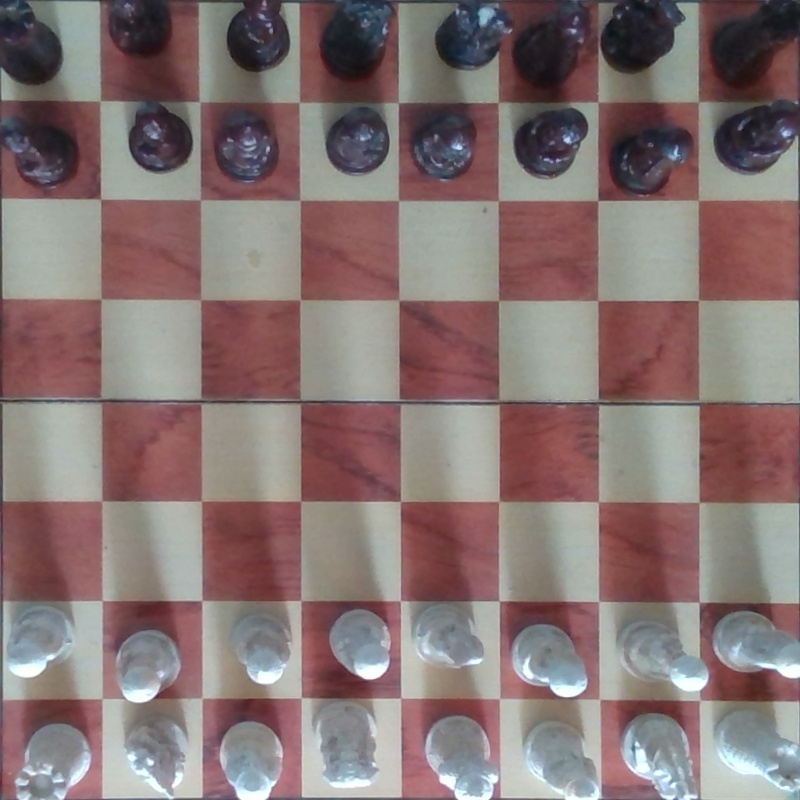
\includegraphics[width=0.19\textwidth]{trail_small_1.jpg} & 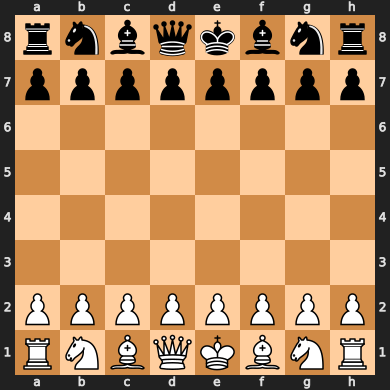
\includegraphics[width=0.19\textwidth]{starting_board.png} & 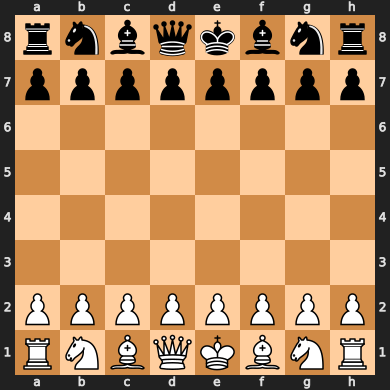
\includegraphics[width=0.19\textwidth]{starting_board.png} & 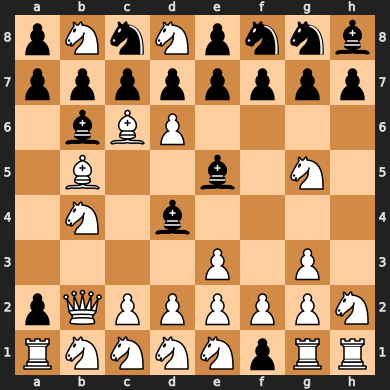
\includegraphics[width=0.19\textwidth]{mym_small_1.png} & 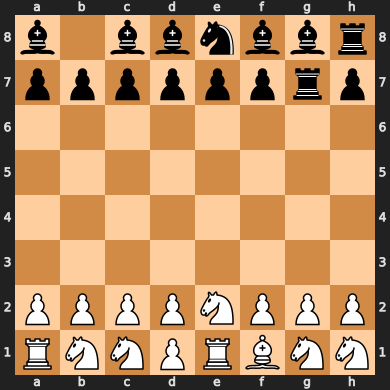
\includegraphics[width=0.19\textwidth]{cv_small_1.png} \\
        & Mistakes: & 0 & 11 & 3 \\
        \hline
        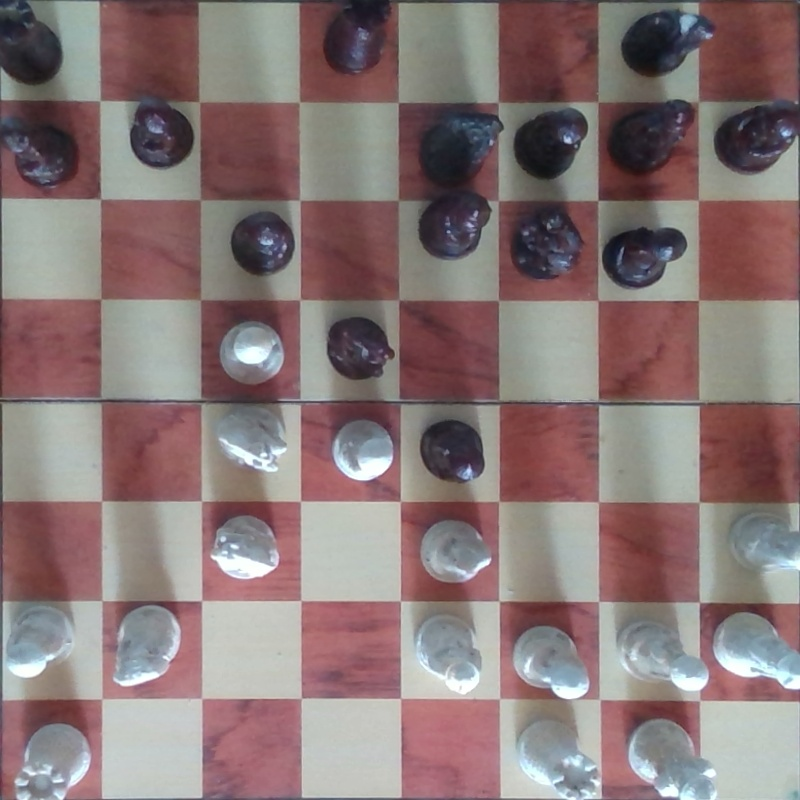
\includegraphics[width=0.19\textwidth]{trail_small_2.jpg} & 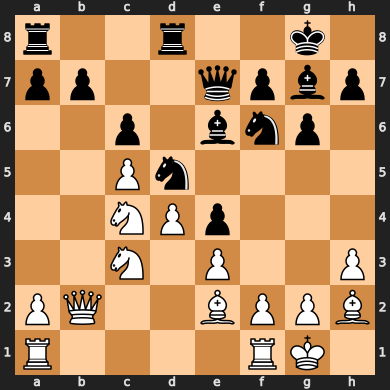
\includegraphics[width=0.19\textwidth]{small_board_2.png} & 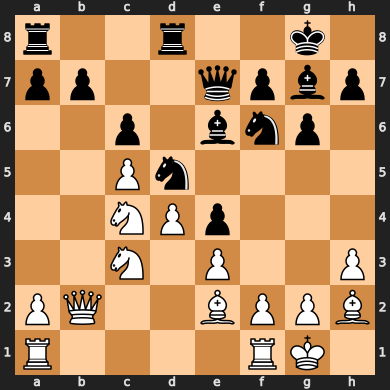
\includegraphics[width=0.19\textwidth]{small_board_2.png} & 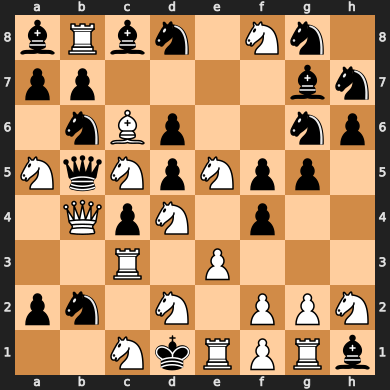
\includegraphics[width=0.19\textwidth]{mym_small_2.png} & 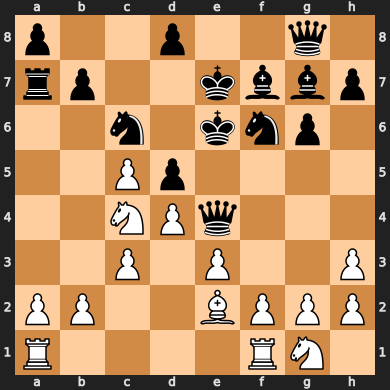
\includegraphics[width=0.19\textwidth]{cv_small_2.png} \\
        & Mistakes: & 0 & 12 & 3 \\
        \hline
        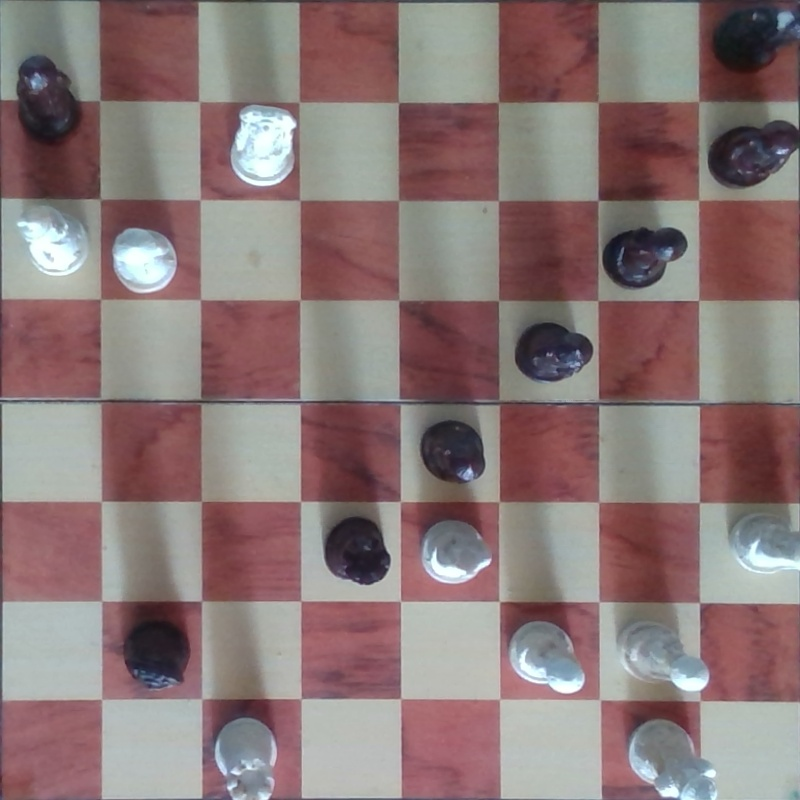
\includegraphics[width=0.19\textwidth]{trail_small_3.jpg} & 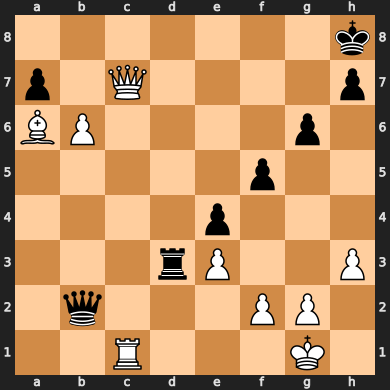
\includegraphics[width=0.19\textwidth]{small_board_3.png} & 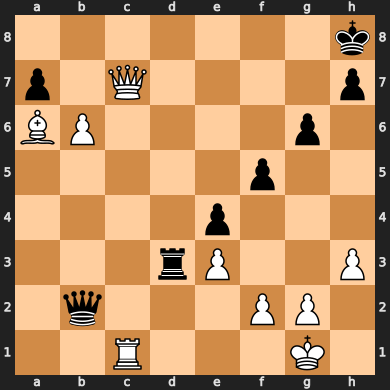
\includegraphics[width=0.19\textwidth]{small_board_3.png} & 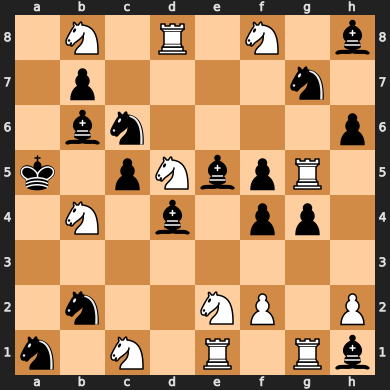
\includegraphics[width=0.19\textwidth]{mym_small_3.png} & 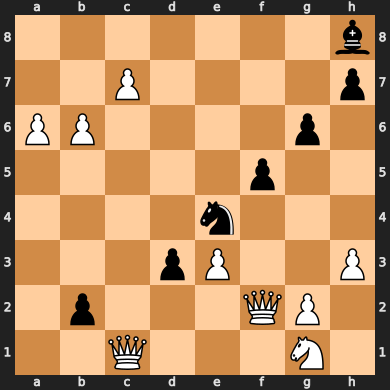
\includegraphics[width=0.19\textwidth]{cv_small_3.png} \\
        & Mistakes: & 0 & 12 & 3 \\
        \hline
        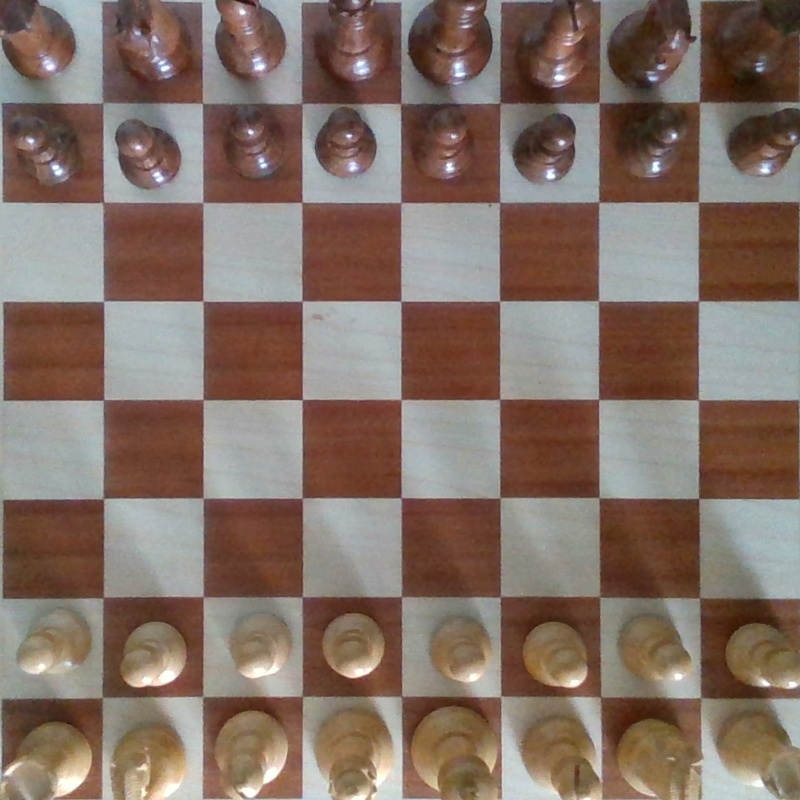
\includegraphics[width=0.19\textwidth]{trail_big_1.jpg} & 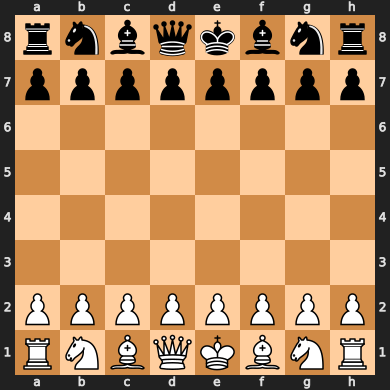
\includegraphics[width=0.19\textwidth]{starting_board.png} & 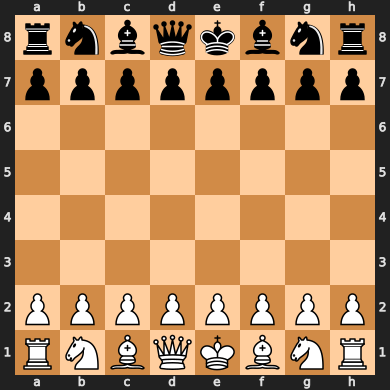
\includegraphics[width=0.19\textwidth]{starting_board.png} & 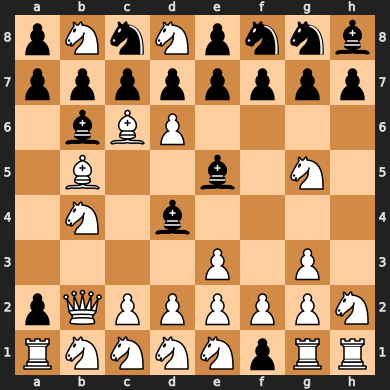
\includegraphics[width=0.19\textwidth]{mym_small_1.png} & 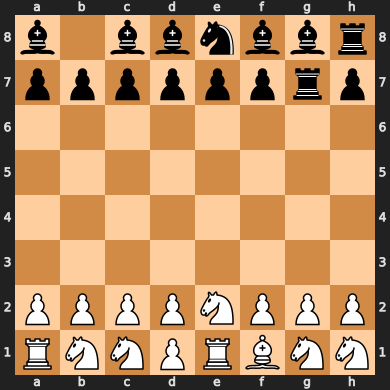
\includegraphics[width=0.19\textwidth]{cv_small_1.png} \\
        & Mistakes: & 0 & 12 & 3 \\
        \hline
        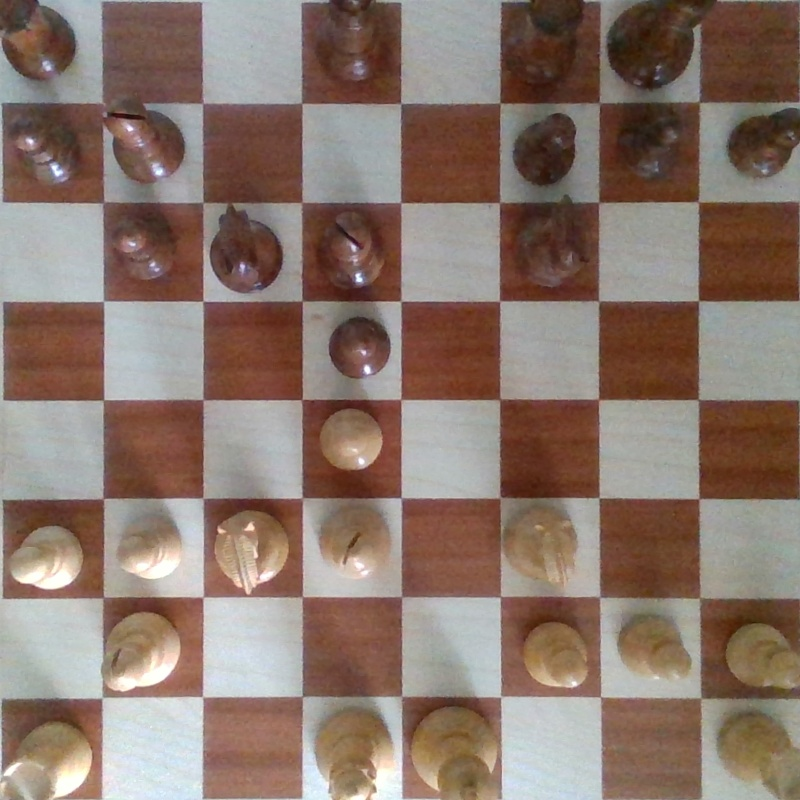
\includegraphics[width=0.19\textwidth]{trail_big_2.jpg} & 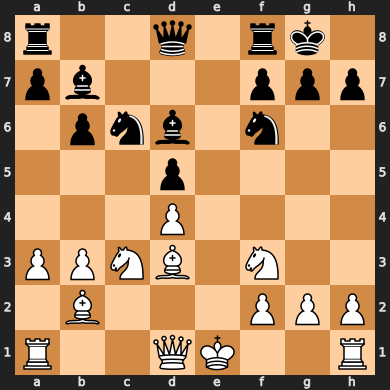
\includegraphics[width=0.19\textwidth]{big_board_2.png} & 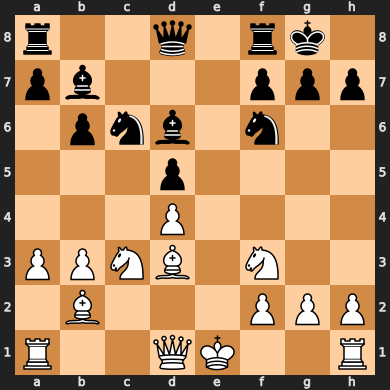
\includegraphics[width=0.19\textwidth]{proposed_big_2.png} & 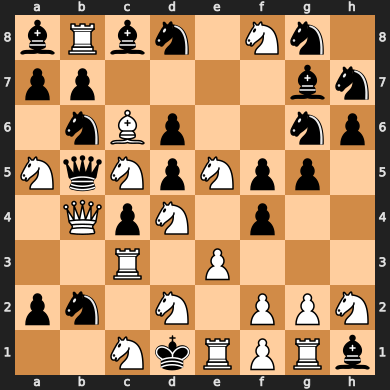
\includegraphics[width=0.19\textwidth]{mym_small_2.png} & 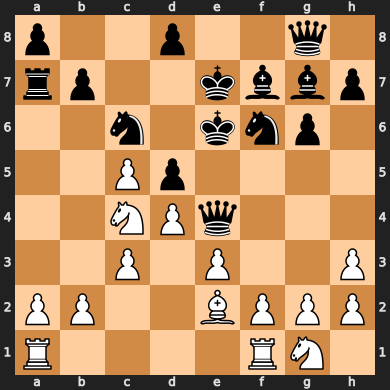
\includegraphics[width=0.19\textwidth]{cv_small_2.png} \\
        & Mistakes: & 0 & 12 & 3 \\
        \hline
        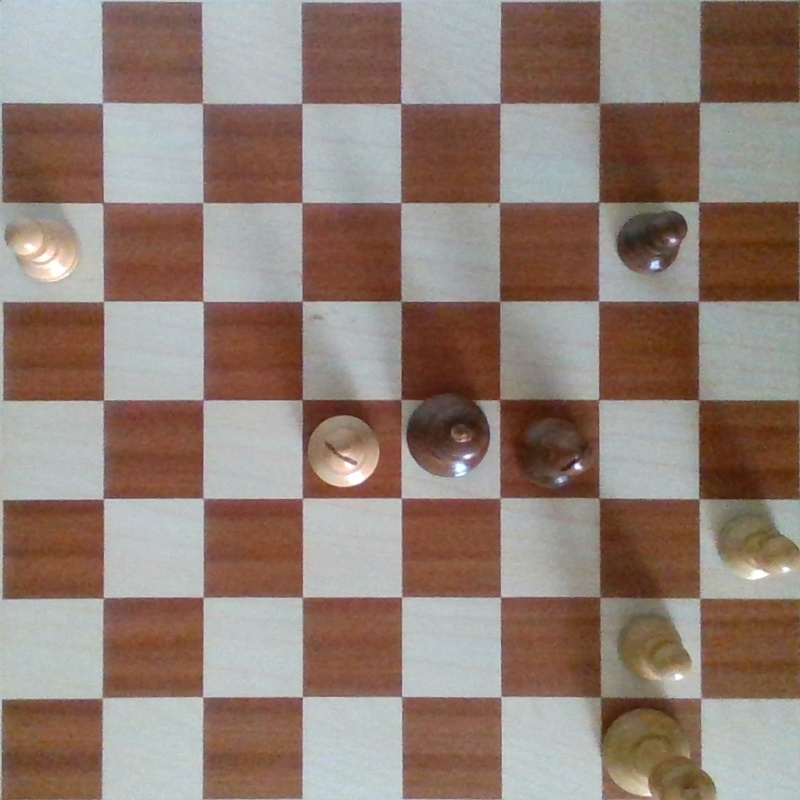
\includegraphics[width=0.19\textwidth]{trail_big_3.jpg} & 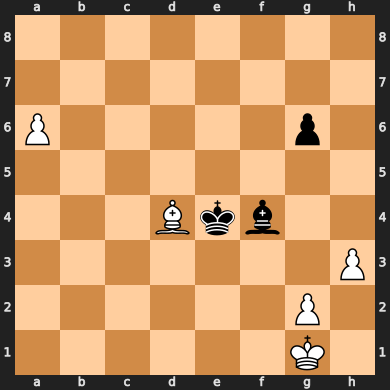
\includegraphics[width=0.19\textwidth]{big_board_3.png} & 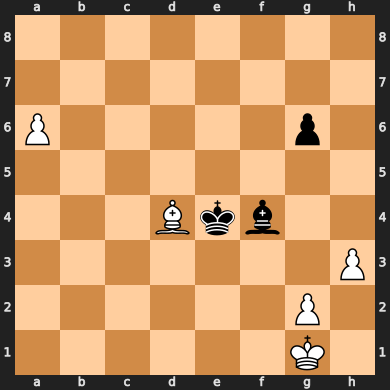
\includegraphics[width=0.19\textwidth]{proposed_big_3.png} & 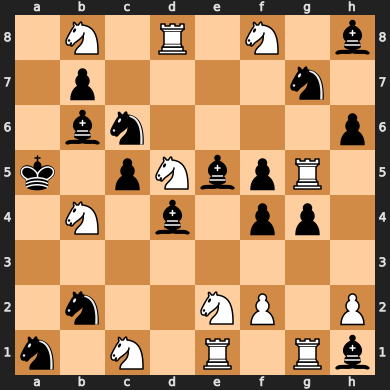
\includegraphics[width=0.19\textwidth]{mym_small_3.png} & 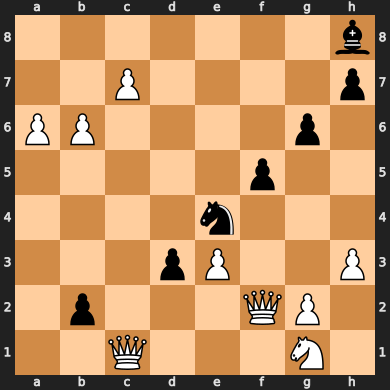
\includegraphics[width=0.19\textwidth]{cv_small_3.png} \\
        & Mistakes: & 0 & 12 & 3 \\
        \hline
    \end{tabu}}
}
\caption{A sample of six segmented chessboard images and their corresponding state prediction from each model}
\label{fig:trails}
\end{figure}


\section{Recording PGN}
\label{evaluate pgn}
In addition to evalutaing the raw model's performance, five games of varying length are played from beginning to end with the inference application.  
The games were played as normal with the only exception being that moves were only made after the inference application detected the previous move.
These delays, as they'll be refereed to in \autoref{fig:games}, were measured with a timer and recorded.  
If the model failed to correctly generate the correct PGN at the end of the game, or otherwise crashed, it was marked as a failure.

\begin{figure}[h]
\centering
\begin{tabular}{|c|c|c|c|c|c|}
    \cline{4-6}
    \multicolumn{3}{c|}{} &  \multicolumn{3}{c|}{Delay for Move to Register (s)} \\
    \hline
    Game & Total Moves & PGN 100\% Correct & Median & Mean & Std Dev \\
    \hline
    Carlsen/Wesley & 57 & \checkmark & 1.25 & 3.01 & 5.26 \\
    Carlsen/Rapport & 36 & \checkmark & 1.13 & 3.21 & 4.97 \\
    Carlsen/Nakamura & 71 & - & 0.95 & 1.82 & 2.09 \\
    Carlsen/Aranian & 55 & \checkmark & 1.24 & 4.20 & 11.31 \\
    Fool's Mate & 4 & \checkmark & 0.95 & 1.19 & 0.76 \\
    \hline
\end{tabular}
\caption{Games played with the inference application}
\label{fig:games}
\end{figure}

The one failed game (Carlsen/Nakamura) was due to the inference application registering a rook movement before the 
player lifted their hand from the rook who then decided to move it to a different square.

The fastest move to register took 0.27s and the slowest took 76s which appeared to be when there 
was lots of specular light reflecting from the pieces causing the model to confuse colors.

\begin{figure}[h]
    \centering
    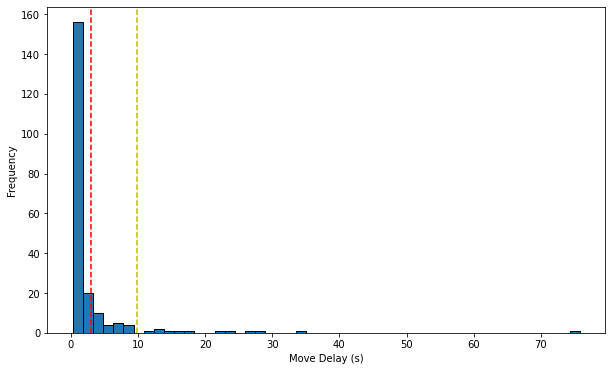
\includegraphics[scale=0.6]{move_delay.png}
    \caption{Histogram of move delay across all games in \autoref{fig:games} with arithmetic mean in red and sample standard deviation in yellow}
\label{fig:delay}
\end{figure}

While the delays on the tail end of the distribution are certainly caused by uncertainty in the model, the cause of the median delay is more difficult to 
pinpoint and so a profiler was used quite a lot through out the project and is shown here in \autoref{fig:profile}.  A reasonable chunk of time is consumed 
by the display function which provides the user feedback as can be seen in the provided demo.  As this is not vital to the function of the application it would 
be possible to place this logic within another thread with a lower priority.  This should completely remove ($\tilde20\%$ of the total delay) if the machine
has a free CPU to schedule the thread to.  Due to using a GPU and inference the entire time spent forward propagating the images through the model took less than 
5\% of the whole inference loop, the most glaring time during inference seems to be spent in the \verb|.item()| method of pytorch which is moving data from the GPU to 
the CPU. 

\begin{figure}[h]
    \centering
    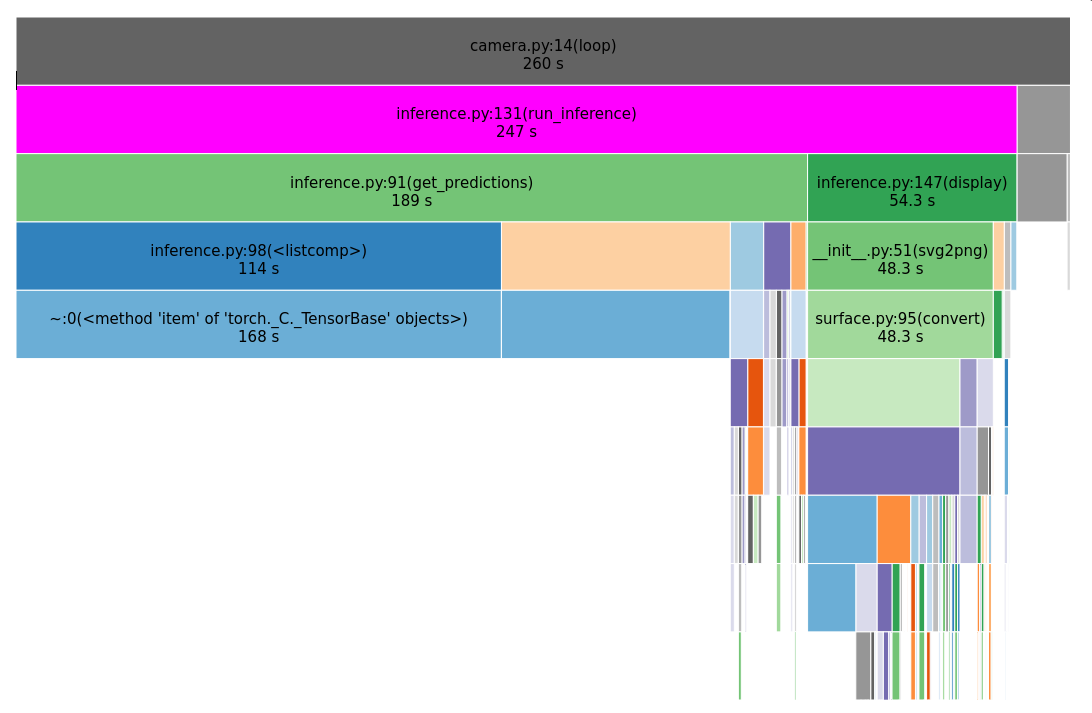
\includegraphics[width=\textwidth]{call_stack.png}
    \caption{cProfile Visualisation of recording a 4 minute game at inference with moves made in quick succession}
    \label{fig:profile}
\end{figure}